\section{Istruzioni di utilizzo}
\subsection{Requisiti hardware}
Trattandosi di una web app, non è richiesto un particolare hardware per farla funzionare, ma è sufficiente un dispositivo con un browser e connesso ad internet. Per sfruttara al meglio questa applicazione è consigliato l'utilizzo da sistemi desktop.

\subsection{Requisiti software}
Per usufruire dell'applicazione SWEDesigner in ambiente desktop è consigliato utilizzare i browser:
\begin{itemize}
\item \emph{Google Chrome}, versione 49.x o superiore;
\item \emph{Mozilla Firefox}, versione 45.y o superiore;
\end{itemize}

\subsection{Prerequisiti}
Per poter utilizzare correttamente l'applicazione non sono richieste particolare conoscenze tecniche, si rimanda alla lettura della sezione successiva nella quale verranno illustrate le principali funzionalità

\subsection{Installazione}
Essendo una applicazione web, non è richiesta alcuna installazione sul proprio dispositivo. Per utilizzarla è necessario effettuare l'accesso con le credenziali fornite in fase di registrazione.

\subsection{Accesso all'applicazione}
Per avere accesso all'applicazione occorre digitare sul proprio browser nella barra degli indirizzi l'URL fornito per l'accesso all'applicazione. Occorrerà inserire i propri dati per l'autenticazione, pertanto sarà necessario effettuare l'operazione di registrazione e solo successivamente sarà possibile effettuare l'operazione di autenticazione.\\
In caso ci si dimentichi la propria password, rimanendo impossibilitati ad effettuare l'autenticazione, sarà possibile ricevere una password temporanea presso il proprio indirizzo email.

\subsubsection{Registrazione}
Dalla pagina iniziale occorre cliccare su \textit{Registrati} e quindi inserire i propri dati all'interno dei campi. Terminato l'inserimento occorre premere il tasto \textit{Registrati}. In caso si desideri ritornare alla pagina iniziale basterà cliccare su \textit{Indietro}.\\
Non sarà possibile cliccare su \textit{Registrati} finché non saranno stati inseriti tutti i dati richiesti e al termine della registrazione verrà effettuata in automatico l'autenticazione.\\
\begin{figure}[H]
	\centering
		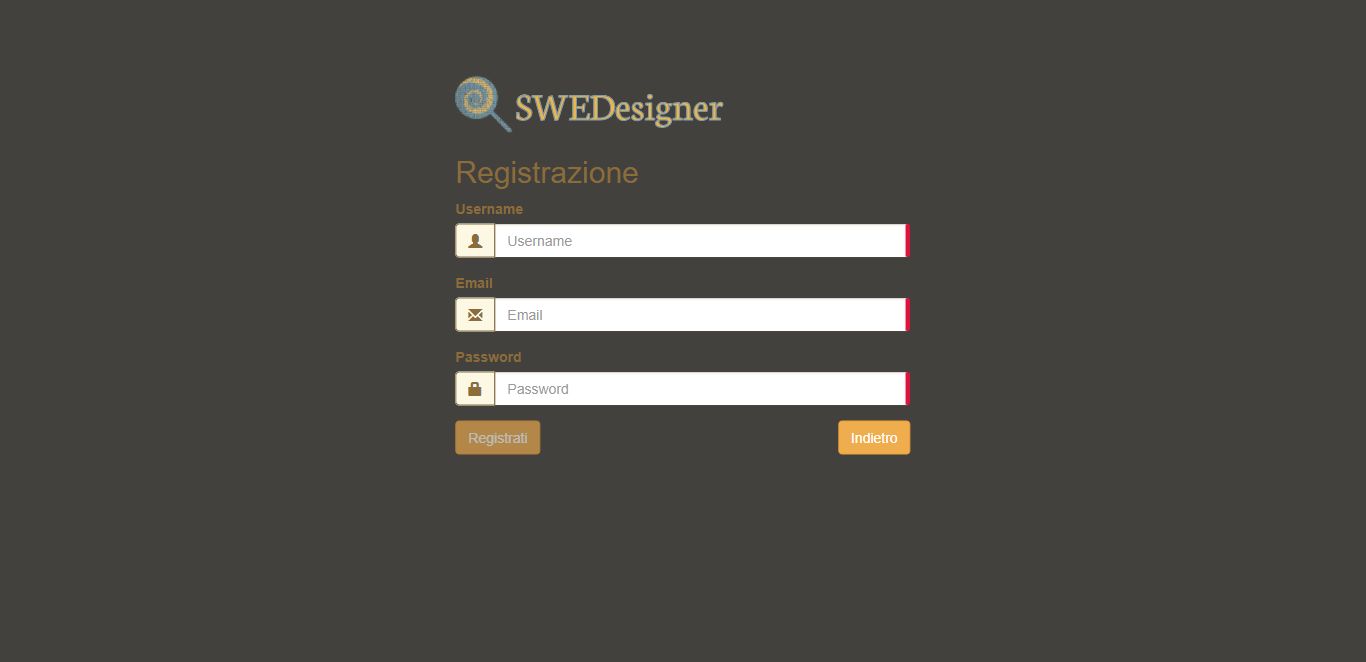
\includegraphics[width=1\linewidth]{res/img/registrazione.png}
	\caption{Pagina di registrazione}
\end{figure}
\newpage

\subsubsection{Autenticazione}
Dopo aver digitato sul proprio browser nella barra degli indirizzi l'URL fornito per l'accesso all'applicazione si aprirà la pagina iniziale, ovvero la pagina di autenticazione.\\
Per effettuare l'autenticazione occorre inserire l'email e la password fornite durante la registrazione e poi cliccare su \textit{Login}.\\
\begin{figure}[H]
	\centering
		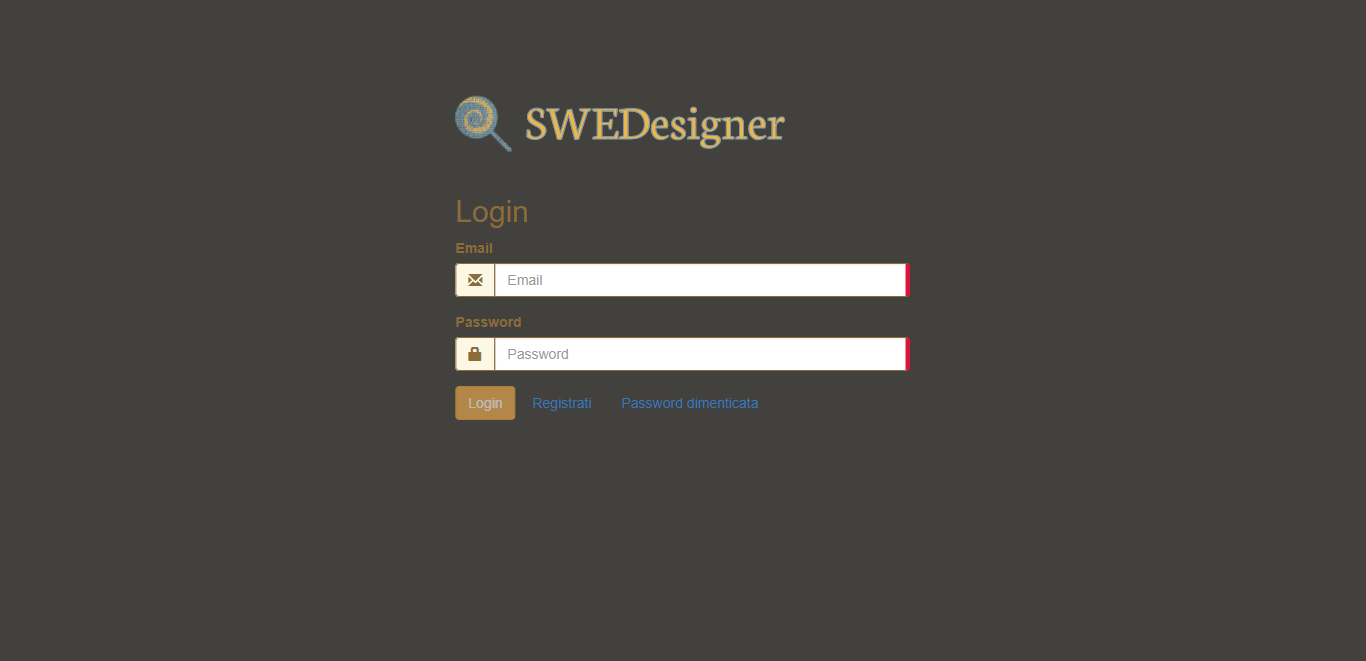
\includegraphics[width=1\linewidth]{res/img/autenticazione.png}
	\caption{Pagina iniziale}
\end{figure}
\newpage

\subsubsection{Recupero password}
In caso non ci si ricordi la password per poter effettuare l'autenticazione, è possibile richiederne una temporanea presso il proprio indirizzo email, fornito durante la registrazione. Per fare ciò occorre, dalla pagina iniziale, cliccare su \textit{Password Dimenticata}, inserire la propria email e cliccare su \textit{Invia}. Se si desidera ritornare alla pagina di autenticazione basterà cliccare su \textit{Indietro}.\\
Non sarà possibile cliccare su \textit{Invia} finché non sarà stata inserita la mail alla quale inviare la password.\\
\begin{figure}[H]
	\centering
		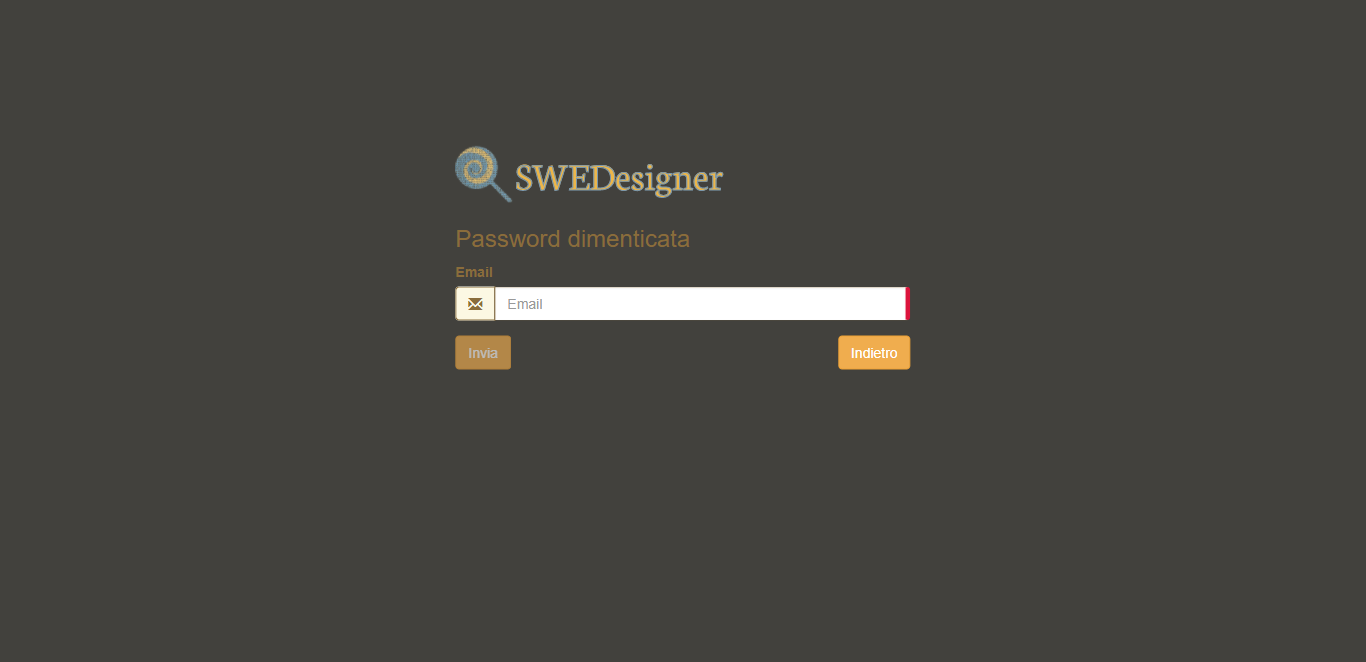
\includegraphics[width=1\linewidth]{res/img/password.png}
	\caption{Pagina di recupero password}
\end{figure}
\newpage